\section{Introduction}

Instruction Level Parallelism (ILP) aims to overlap individual machine operations, such as additions, multiplications, and loads, allowing them to execute in parallel. 
This process is designed to be transparent to the user, with the primary goal of speeding up execution.

In contrast, parallel processing involves using separate processors to handle different chunks of a program, with each processor programmed to perform its tasks independently. 
This method is nontransparent to the user, and it aims to improve both the speed and quality of execution.
To achieve performance improvements beyond a single cycle per instruction (CPI) using parallel processing, we can employ techniques such as Superscalar architecture or Very Long Instruction Word.

\subsection{Very Long Instruction Words}
VLIW architecture uses a fixed number of instructions, typically ranging from 4 to 16, which are scheduled by the compiler and placed into wide templates. 
This approach has found notable success in digital signal processing (DSP) and multimedia applications.
A significant milestone in VLIW development was the joint agreement between HP and Intel in 1999/2000, leading to the creation of the Intel Architecture-64 (Merced/A-64) with a 64-bit address space. 
This style of architecture is known as an Explicitly Parallel Instruction Computer (EPIC).

A processor can initiate multiple operations per cycle, with all operations specified entirely by the compiler, unlike in Superscalar architectures. 
This approach results in low hardware complexity as there is no need for scheduling hardware and reduced support for variable latency instructions. 
Additionally, the hardware does not perform any instruction reordering, ensuring explicit parallelism and a single control flow.

In this context, an operation refers to a unit of computation, such as an addition, load, or branch, similar to an instruction in a sequential architecture. 
An instruction, however, is a set of operations intended to be issued simultaneously. 
The compiler decides which operations go into each instruction through scheduling. 
All operations that are supposed to start at the same time are packaged into a single VLIW instruction.

Multiple operations are packed into one instruction, with each operation slot designated for a specific function. 
Constant operation latencies are specified, and the architecture requires a guarantee of parallelism within an instruction, meaning there is no need for cross-operation read-after-write (RAW) checks. 
Furthermore, no data is used before it is ready, eliminating the need for data interlocks.
\begin{figure}[H]
    \centering
    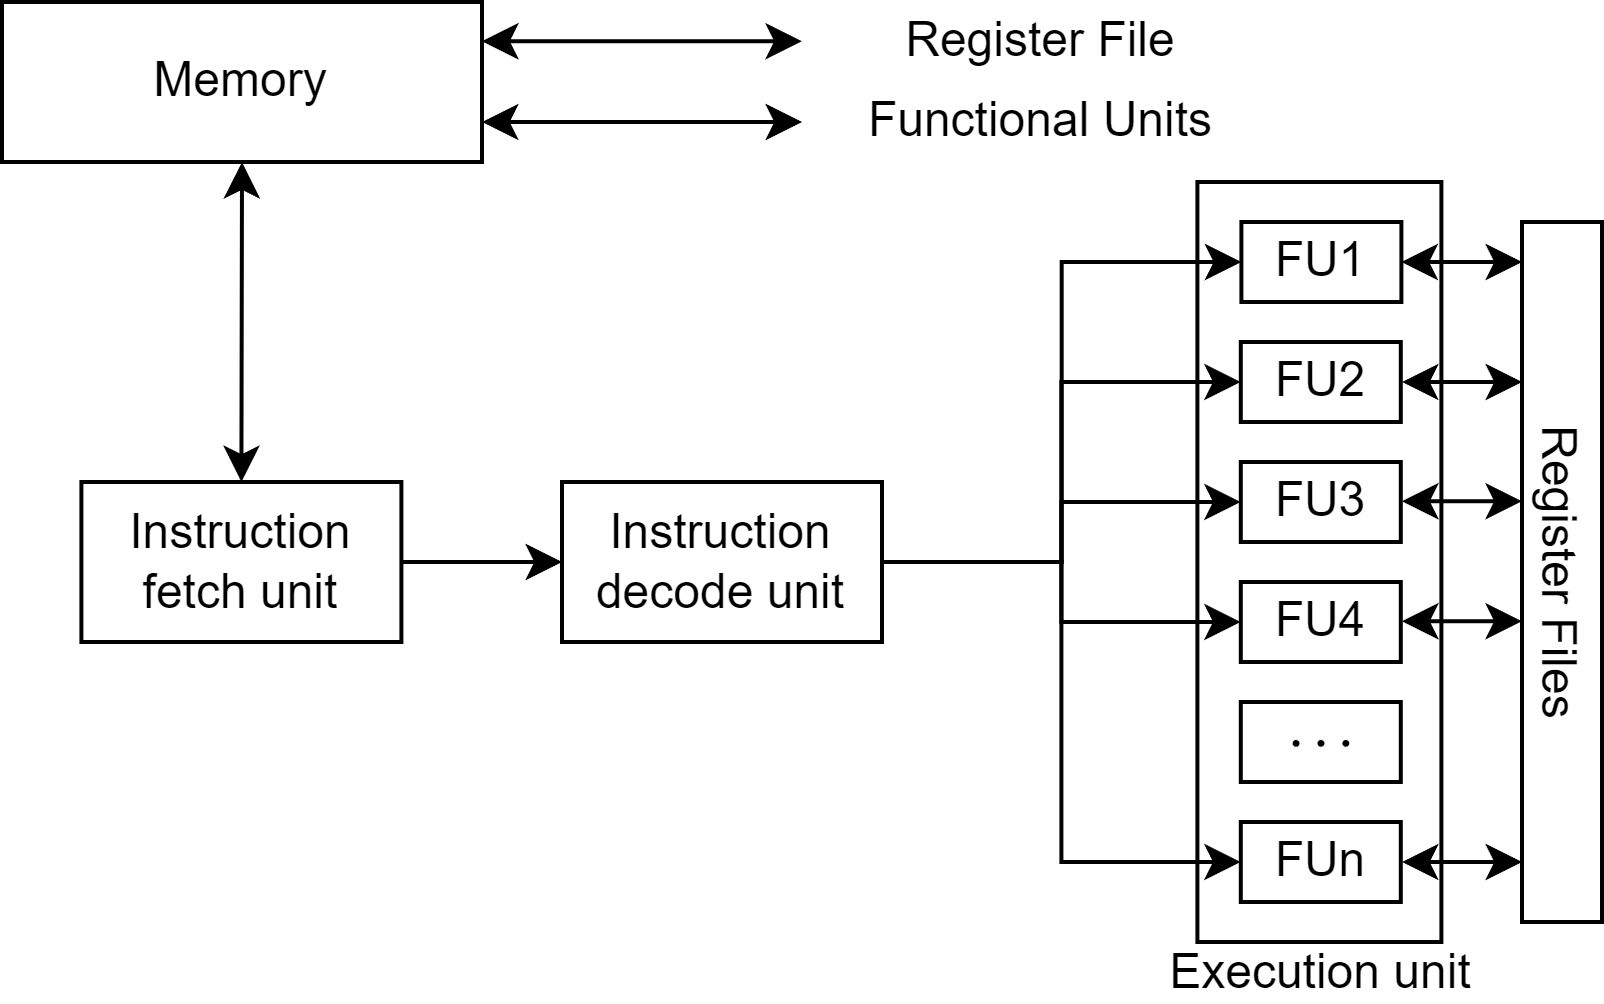
\includegraphics[width=0.75\linewidth]{images/vliw.png}
    \caption{VLIW machine configuration}
\end{figure}